\chapter{Introduction}
\section{Polynomial Constraint Solving}
{\em Polynomial constraint solving over real numbers} aims at computing an assignment of real values to variables
that satisfies given polynomial inequalities/equations. If such an assignment exists, the constraint is said to be satisfiable (SAT) and the assignment is called SAT instance; otherwise we mention it as unsatisfiable (UNSAT). 
\begin{example} \label{examp:unsat-example}
The constraint $x^2 + y^2 < 1 \wedge xy > 1$ is an example of an unsatisfiable one. While the set of satisfiable points for the first inequality ($x^2 + y^2 < 1$) forms the read circle in Figure \ref{fig:unsat-example}, that for the second forms the blue area. Because these two areas do not intersect, the conjunction of two inequalities is unsatisfiable.
\end{example}

\begin{figure}[ht]
%\begin{minipage}[b]{1.0\linewidth}
\centering
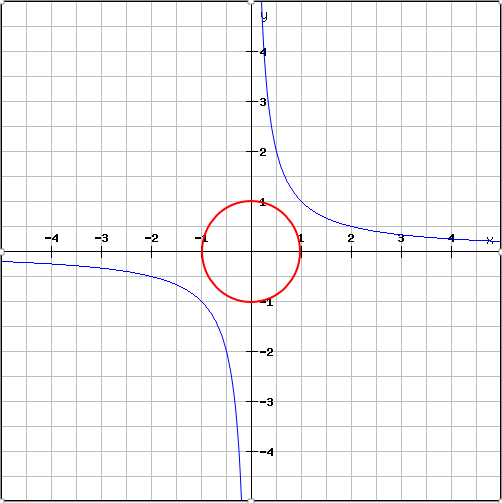
\includegraphics[scale = 0.5]{UNSAT-example.png} 
\caption{Example of UNSAT constraint} 
\label{fig:unsat-example} 
%\end{minipage}
\end{figure} 

\begin{example} \label{examp:sat-example} \sloppy
Figure~\ref{fig:sat-example} illustrates the satisfiability of the constraint: ${x^2 + y^2 < 4 \wedge xy > 1}$. Any point in the purple area is a SAT instance of the constraint, e.g. $(1.5, 1)$.
\end{example}

\begin{figure}[ht]
%\begin{minipage}[b]{1.0\linewidth}
\centering
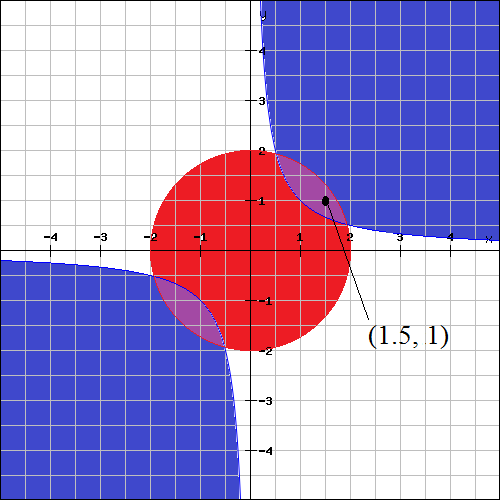
\includegraphics[scale=0.5]{SAT-example.png} 
\caption{Example of SAT constraint} 
\label{fig:sat-example} 
%\end{minipage}
\end{figure} 

%For instance, $\exists x y. -y^2 + (x^2 - 1) y - 1 > 0 \wedge -x^2 - y^2 + 4 > 0$ is 
%such an example. This is an easy formula, but proving its satisfiability and 
%showing a satisfiable instance (e.g., $x = 1.8$, $y=0.9$) are not so easy.  
%its satisfiability and a satisfiable instance 
%(e.g., $x = 1.8$, $y=0.9$) are not so easy.  		
%
Solving polynomial constraints has many application in Software Verification, such as 
\begin{itemize}
\item[$\bullet$] {\bf Locating roundoff and overflow errors}
which is our motivation~\cite{Ngoc:2009:ORE:1685167.1685421,Ngoc:2010:CRE:1858996.1859056}.
%DSP decorders in practice are defined by reference algorithms in C using floating point arithmetic. 
%In embedded systems, often it is replaced with fixed point arithmetic, 
%which may cause visible noises. 
%and locating such roundoff error source is not easy. 
%For instance, consider DSP decoder like mpeg4. Usually, the decoder definition is given by a reference 
%algorithm in C, which uses floating point number. 
%In an embedded system, it is tempting to replace floating 
%point into fixed point numbers. However, naive replacement would cause 

\item[$\bullet$] {\bf Automatic termination proving} 
which reduces termination detection to finding a suitable ordering~\cite{Lucas:2008:CCS:1361735.1361760}, 
e.g., \TTTT\footnote{\url{http://cl-informatik.uibk.ac.at/software/ttt2/}}, 
AProVE\footnote{\url{http://aprove.informatik.rwth-aachen.de}}, that leads to polynomial constraints. 
%as a solution of polynomial constraints. 

\item[$\bullet$] {\bf Loop invariant generation}~\cite{Colon,Sankaranarayanan:2004:NLI:982962.964028} is reduced to solving polynomial constraints over coefficients of invariant template. 
%matrix multiplications. 
%degree $2$ polynomial constraints. 
%Farkas's lemma uses products of matrices, and it requires solving polynomial constraints of degree 2.
%Non-linear loop invariant~\cite{Sankaranarayanan:2004:NLI:982962.964028} requires more complex polynomials.

\begin{comment}
\item {\bf Hybrid system}. Solving polynomial constraints over real numbers is often used as backend engines~\cite{Sankaranarayanan04constructinginvariants}. 

\item {\bf Mechanical contrnol design}. 
PID control is simple but widely used, and designing parameters is 
reduced to polynomial constraints~\cite{control}. 
%Fujitsu used polynomial constraints solving to design PID control of HDD head movement
\end{comment}
\end{itemize}	

\section{Existing Approaches}
Although solving polynomial constraints on real numbers is decidable~\cite{tarski}, current methodologies have their own pros and cos. They can be classified into the following categories: 
\begin{enumerate}
\item \textbf{Quantifier Elimination by Cylindrical Algebraic Decomposition (QE-CAD)}~\cite{qecad} 
is a complete technique, and 
is implemented in Mathematica, Maple/SynRac, Reduce/Redlog, QEPCAD-B, and recently 
in
Z3 4.3 (which is referred as nlsat in~\cite{Jovanovic13}).
Although QE-CAD is precise and detects beyond SAT instances (e.g., SAT regions), 
scalability is still challenging, since its complexity is doubly-exponential with respect to the number of variables. 
%Since QE-CAD is DEXPTIME wrt the number of variables, 

\item \textbf{Virtual Substitution } eliminates an existential quantifier by substituting the corresponding quantified variable with a very small value ($-\infty$), and either each root (with respect to that variable) of polynomials appearing in the constraint or each root plus an infinitesimal $\epsilon$. Disjunction of constraints after substitutions is equivalent to the original constraint. Because VS needs the formula for roots of polynomials, its application is restricted to polynomials of degree up to 4. SMT-RAT and  
Z3 \cite{PBM12} applies VS.

\item \textbf{Bit-blasting}. 
In this category of methodology, numerical variables are represented by a sequence of binary variables. The given constraint is converted into another constraint over the boolean variables. SAT solver is then used to find a satisfiable instance of binary variables which can be used to calculate the values of numerical variables.  MiniSmt~\cite{Zankl:2010:SNR:1939141.1939168}, the winner of QF\_NRA in SMT competition 2010, 
applies it for (ir)-rational numbers.
It can show SAT quickly, but due to the bounded bit encoding, 
it cannot conclude UNSAT. In addition, high degree of polynomial results in large SAT formula which is an obstacle of bit-blasting.

\item \textbf{Linearization}. ~
CORD \cite{cordic} uses COrdinate Rotation DIgital Computer (CORDIC) for real numbers to linearizes multiplications into a sequence of linear constraints. Each time one multiplication is linearized, a number of new constraints and new variables are introduced. As a consequence, high degree polynomials in the original constraint lead to large number of linear constraints. 

\item \textbf{Interval Constraint Propagation (ICP)} 
which are used in SMT solver community, e.g., iSAT3~\cite{isat}, 
dReal~\cite{dRealCADE13}, and RSOLVER~\cite{rsolver}. 
ICP combines over-approximation by interval arithmetics and constraint propagation to prune out the set of unsatisfiable points. When pruning does not work, decomposition (branching) on intervals is applied. 
ICP which is capable of solving "multiple thousand arithmetic constraints over some thousands of variables" \cite{isat} is practically often more efficient than algebraic computation.
\end{enumerate}

\section{Proposed Approach and Contributions}
Our aim is an SMT solver for solving polynomial constraint. We first focus on strict inequalities because of the following reasons.
\begin{enumerate}
\item
Satisfiable inequalities allow over-approximation. An over-approximation estimates the range of a polynomial $f$ as $range_O(f)$ that covers all the possible values of $f$, i.e. $range(f) \subseteq range_O(f)$. For an inequality $f>0$, if $range_O(f)$ stays in the positive side, it can be concluded as SAT. On the other hand, over-approximation cannot prove the satisfiability of SAT equations.
\item
Satisfiable inequalities allow under-approximation. An under-approximation computes the range of the polynomial $f$ as  $range_U(f)$ such that $range(f) \supseteq range_U(f)$. If $range_U(f)$ is on the positive side, $f > 0$ can be said to be SAT. Due to the continuity of $f$, finding such an under-approximation for solving $f > 0$ is more feasible than that for $f = 0$.
\begin{itemize}
\item[$\bullet$] If $f(\bar{x}) > 0$ has a real solution $\bar{x}_0$, there exist rational points near $\bar{x}_0$ which also satisfy the inequality. Solving inequalities over real numbers thus can be reduced to that over rational numbers.
\item[$\bullet$] The real solution of $f(\bar{x}) = 0$ cannot be approximated to any rational number.
\end{itemize}
\end{enumerate}
For UNSAT constraint (both inequalities and equations) can be solved by over-approximation. Suppose $range_O(f)$ is the result of an over-approximation for a polynomial $f$.
\begin{enumerate}
\item If $range_O(f)$ resides on the negative side, $f > 0$ is UNSAT.
\item If $range_O(f)$ stays on either negative or positive side, $f = 0$ is UNSAT.
\end{enumerate}

Our approach of "iterative approximation refinement" - \textbf{raSAT} loop for solving polynomial constraint was proposed and implemented as an SMT solver named raSAT in \cite{VanKhanh201227}. This work improves the efficiency of the tool and extend it to handle equations and constraints over integer numbers. The summary of the proposed method in \cite{VanKhanh201227} is:
\begin{enumerate}
\item \emph{Over-approximation} is used for both disproving and proving polynomial inequalities. In addition, \emph{under-approximation} is used for boosting SAT detection. When both of these methods cannot conclude the satisfiability, the input formula is \emph{refined} so that the result of approximation become more precise. 
\item \emph{Interval Arithmetic} (IA) and \emph{Testing} are instantiated as an over-approximation and an under-approximation respectively. While IA defines the computations over the intervals, e.g. $[1, 3] +_{IA} [3, 6] = [2, 9]$, Testing attempts to propose a number of assignments of real numbers to variables and check each assignment against the given constraint to find a SAT instance.
\item In \emph{refinement} phase, intervals of variables are decomposed into smaller ones. For example, $x \in [0, 10]$ becomes $x \in [0, 4] \vee x \in [4, 10]$.
\item \citet{VanKhanh201227} also proposed a method for detecting \emph{satisfiability of equations} using the Intermediate Value Theorem.
\end{enumerate}

The contributions of this work are as follows:
\begin{enumerate}
\item Although the method of using IA is robust for large degrees of polynomial, the number of boxes (products of intervals) grows exponentially with respect to the number of variables during refinement (interval decomposition). As a result, strategies for \emph{selectin gone variable} to decomposed and \emph{selecting one box} to explore play a crucial role in efficiency. We introduce the following strategies:
\begin{itemize}
\item[$\bullet$] \textbf{Selecting one box.} The box with more possiblity to satisfy the constraint is selected to explore, which is estimated by 
several heuristic measures, called {\em SAT likelyhood}, 
and \emph{the number of unsolved polynomial inequalities}.
\item[$\bullet$] \textbf{Selecting one variable.} The most influential variable is selected for multiple test cases and decomposition. 
This is estimated by {\em sensitivity} which is determined during the computation of IA.
\end{itemize}
\item Two schemes of \emph{incremental search} are proposed for enhancing solving process: 
\begin{itemize} 
\item[$\bullet$] {\bf Incremental deepening}. 
raSAT follows the depth-first-search manner. In order to escape local optimums, it starts searching with a threshold that each interval will be decomposed no smaller than it. 
If neither SAT nor UNSAT is detected, a smaller threshold is taken and raSAT restarts. 
\item[$\bullet$] {\bf Incremental widening}. 
Starting with a small interval, if \textbf{raSAT} detects UNSAT, input intervals are enlarged
and raSAT restarts. For SAT constraint, small (finite) interval allows sensitivity to be computed because Affine Interval \cite{VanKhanh201227} requires finite range of variables. As a consequence, our above strategies will take effects on finding SAT instance. For the UNSAT case, combination of small intervals and incremental deepening helps \textbf{raSAT} quickly determines the threshold in which unsatisfiability may be proved by IA. 
\end{itemize} 
\begin{comment}
SAT-likelihood is introduced to measure the possibility of an inequality to be satisfiable. Sensitivity is proposed to estimate the influence of a variable to the value of a polynomial.
\end{comment}
\item \emph{SAT confirmation} step by an error-bound guaranteed floating point package {\bf iRRAM}\footnote{% 
\tt http://irram.uni-trier.de}, to avoid soundess bugs caused by roundoff errors.
\item This work also implemented the idea of using Intermediate Value Theorem to show \emph{the satisfiability of multiple equations} which was suggested in \cite{VanKhanh201227}.
\item We also extend raSAT to \emph{handle constraints over integer numbers}. For this extension, we only generate the integer values for variables in testing phase. In addition, the threshold used for stopping decomposition is set to $1$.
\end{enumerate}
\begin{comment}
\subsection{Inequalities}
Constraints with inequalities can be categorized into four cases:
\begin{enumerate}
\item \textbf{SAT with without touching}
\begin{figure}[ht]
%\begin{minipage}[b]{1.0\linewidth}
\centering
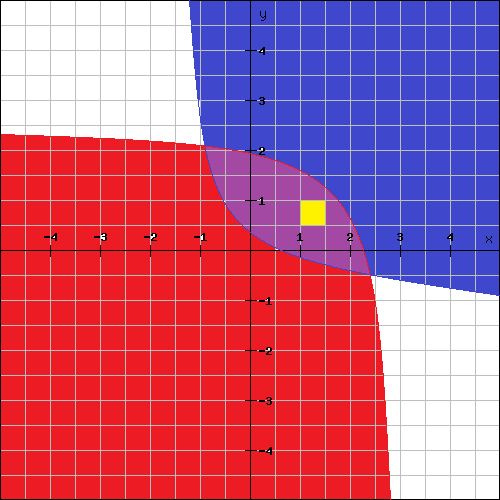
\includegraphics{SAT-withoutTouching.png} 
\caption{SAT without touching dectected by ICP} 
\label{fig:sat-withoutTouching} 
%\end{minipage}
\end{figure} 

\item \textbf{SAT/UNSAT with touching/convergence}
\begin{figure}[ht]
%\begin{minipage}[b]{1.0\linewidth}
\centering
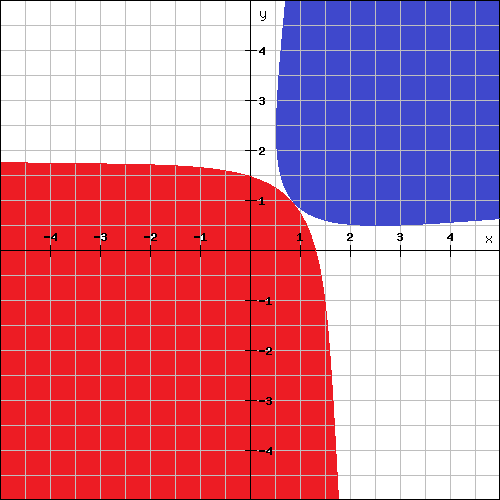
\includegraphics{SAT-touching.png} 
\caption{SAT(UNSAT) detected by Grobner basis method} 
\label{fig:sat-touching} 
%\end{minipage}
\end{figure} 

\item \textbf{UNSAT without touching/convergence}
\begin{figure}[ht]
%\begin{minipage}[b]{1.0\linewidth}
\centering
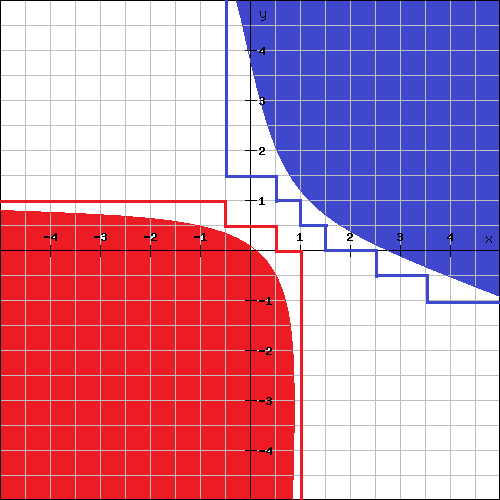
\includegraphics{UNSAT-withoutTouching.png} 
\caption{UNSAT detected by ICP} 
\label{fig:unsat-withoutTouching} 
%\end{minipage}
\end{figure} 
\end{enumerate}
\end{comment}
\begin{comment}
$\exists x_1 \in (a_1,b_1) \cdots x_n \in (a_n,b_n) . \wedge_{i} f_i > 0$, 
\begin{itemize}
\item If $\exists x_1 \in (a_1,b_1) \cdots x_n \in (a_n,b_n) . \wedge_{i} f_i > 0$ is SAT, 
ICP eventually detects it. 
\item If $\exists x_1 \in [a_1,b_1] \cdots x_n \in [a_n,b_n] . \wedge_{i} f_i \geq 0$ is UNSAT, 
ICP eventually detects it
\end{itemize}
under the assumptions of {\em fair} decomposition and bounded intervals. 
\begin{figure}[ht]
%\begin{minipage}[b]{1.0\linewidth}
\centering
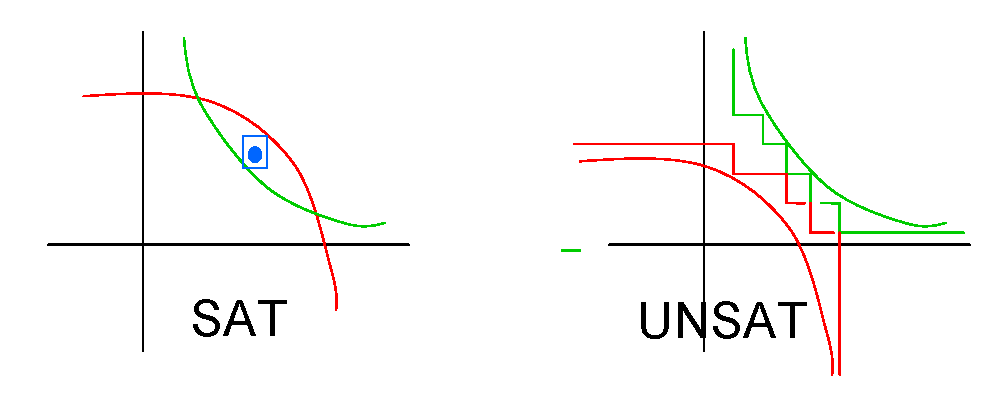
\includegraphics[height=1.2in,width=3.4in]{FigCompleteness.eps} 
\caption{SAT and UNSAT detection by ICP} 
\label{fig:complete} 
%\end{minipage}
\end{figure} 

The boundary part is reduced to polynomial equality checking, 
which would be solved algebraic methods, like Groebner basis. 
Alternatively, by loosening equality to $\delta$-equality, 
$\delta$-completeness is obtained~\cite{dRealIJCAR12,dRealLICS12}. 

This paper presents an SMT solver {\bf raSAT} for polynomial inequality. 
It consists of a simple iterative approximation refinement, called {\bf raSAT} {\em loop}, 
which is an extension of the standard ICP with testing to accelerate SAT detection. 
Two approximation schemes consist of interval arithmetic (over-approximation) and 
testing (under-approximation), to accelerate SAT detection. 
If both fails, input intervals are refined by decomposition. 
%
Compared to typical ICPs, {\bf raSAT} 
\begin{itemize}
\item introduces testing (as an under-approximation) to accelerate SAT detection, 
\item applies various interval arithmetic, e.g., Affine intervals~\cite{Stolfi03,ngocase,tapas12}, 
which enables to analyze the effects of input values, and 
\item SAT confirmation step by an error-bound guaranteed floating point package {\bf iRRAM}\footnote{% 
\tt http://irram.uni-trier.de}, to avoid soundess bugs caused by roundoff errors. 
\end{itemize}
This design is more on SAT detection oriented, since from our preliminary experiences, 
if the target problems have several hundred variables, solvable cases in practice are 
either SAT or UNSAT with small UNSAT core. 
Thus, acceleration of SAT detection and finding UNSAT core will be keys for scalability. 

ICP is robust for larger degrees, but the number of boxes (products of intervals) to explore 
exponentially explodes when variables increase. 
Thus, design of strategies for selecting variables to decompose and boxes to explore is crucial 
for efficiency. Our strategy design is, 
\begin{itemize}
\item a box with more possiblity to be SAT is selected to explore, which is estimated by 
several heuristic measures, called {\em SAT likelyhood}, 
and the number of unsolved atomic polynomial constraints, and
\item a more influential variable is selected for multiple test cases and decomposition, 
which is estimated by {\em sensitivity}. 
\end{itemize} 
Note that {\em SAT likelyhood} and {\em sensitivity} are estimated during interval arithmetic. 
Especially, the latter can be applied only with Affine intervals. 
{\bf raSAT} also applies incremental search, which is often faster in practice. 
\begin{itemize}
\item {\bf Incremental widening}. 
Starting {\bf raSAT} loop with a smaller interval, and if it is UNSAT, enlarge the input intervals
and restart. 
\item {\bf Incremental deepening}. 
Starting with the bound that each interval will be decomposed no smaller than it. 
If neither SAT nor UNSAT is detected, take a smaller bound and restart. 
\end{itemize} 
Efficient UNSAT core and UNSAT confirmation % with error bound guaranteed floating point arithmetic 
are left for future work. 

They are compared on Zankl and Meti-Tarski benchmarks from 
QF\_NRA category of SMT-LIB\footnote{\tt http://www.smtlib.org/}. 
They are also evaluated by comparing 
{\bf Z3 4.3}\footnote{\tt http://z3.codeplex.com} and {\bf iSAT3}. 
Another advantage of {\bf raSAT} is the ease to handle mixed intergers, 
and experiments on AProVE benchmark from QF\_NIA category of SMT-LIB compares {\bf raSAT} with 
{\bf Z3 4.3}. 
Although {\bf Z3 4.3} performs the best, {\bf raSAT} shows comparable SAT detection on 
very large problems (e.g., with several hundred variables) with the combination of 
{\em SAT likelyhood} and {\em sensitivity}. 


\medskip 
{\bf raSAT} applies SAT confirmation to avoid soundness errors caused by roundoff/overflow errors. 
Another static analysis based approach is found in~\cite{SilvaTACAS12}. 
\end{comment}

\section{Thesis Outline}
Coming soon...